\documentclass{theozettel}

%%%%%%%%%%%%%%%%%%%%%%%%%%%%%%%%%%%%%%%%%%%%%%%%%%%%%%%%%%%%%%%%%%%%%%%%%%%%%%%%%%%%%%%%%%%%%%%%%%%%%%%%%%%%%%
% page geometry
%%%%%%%%%%%%%%%%%%%%%%%%%%%%%%%%%%%%%%%%%%%%%%%%%%%%%%%%%%%%%%%%%%%%%%%%%%%%%%%%%%%%%%%%%%%%%%%%%%%%%%%%%%%%%%
\geometry{
	left=20mm,
	right=20mm,
	top=25mm,
	bottom=20mm
}
%%%%%%%%%%%%%%%%%%%%%%%%%%%%%%%%%%%%%%%%%%%%%%%%%%%%%%%%%%%%%%%%%%%%%%%%%%%%%%%%%%%%%%%%%%%%%%%%%%%%%%%%%%%%%%

\pgfplotsset{compat=1.16}

%\renewcommand{\phi}{\varphi}

\usepackage{parskip}
\usepackage{dsfont}
\newcommand{\difd}{\text{d}}
\usepackage{titlesec} 
\titleformat{\section}[runin]
{\normalfont\large\bfseries}{\thesubsection}{1em}{}
\titleformat{\subsection}[runin]
  {\normalfont\normalsize\bfseries}{\thesubsubsection}{1em}{}
  
\renewcommand{\epsilon}{\varepsilon}
\newcommand{\vol}{\operatorname{vol}}

\theoI{8}

\begin{document}
\punkteV{8.1}{8.2}{8.3}{8.4}

\section*{Aufgabe 8.1} 

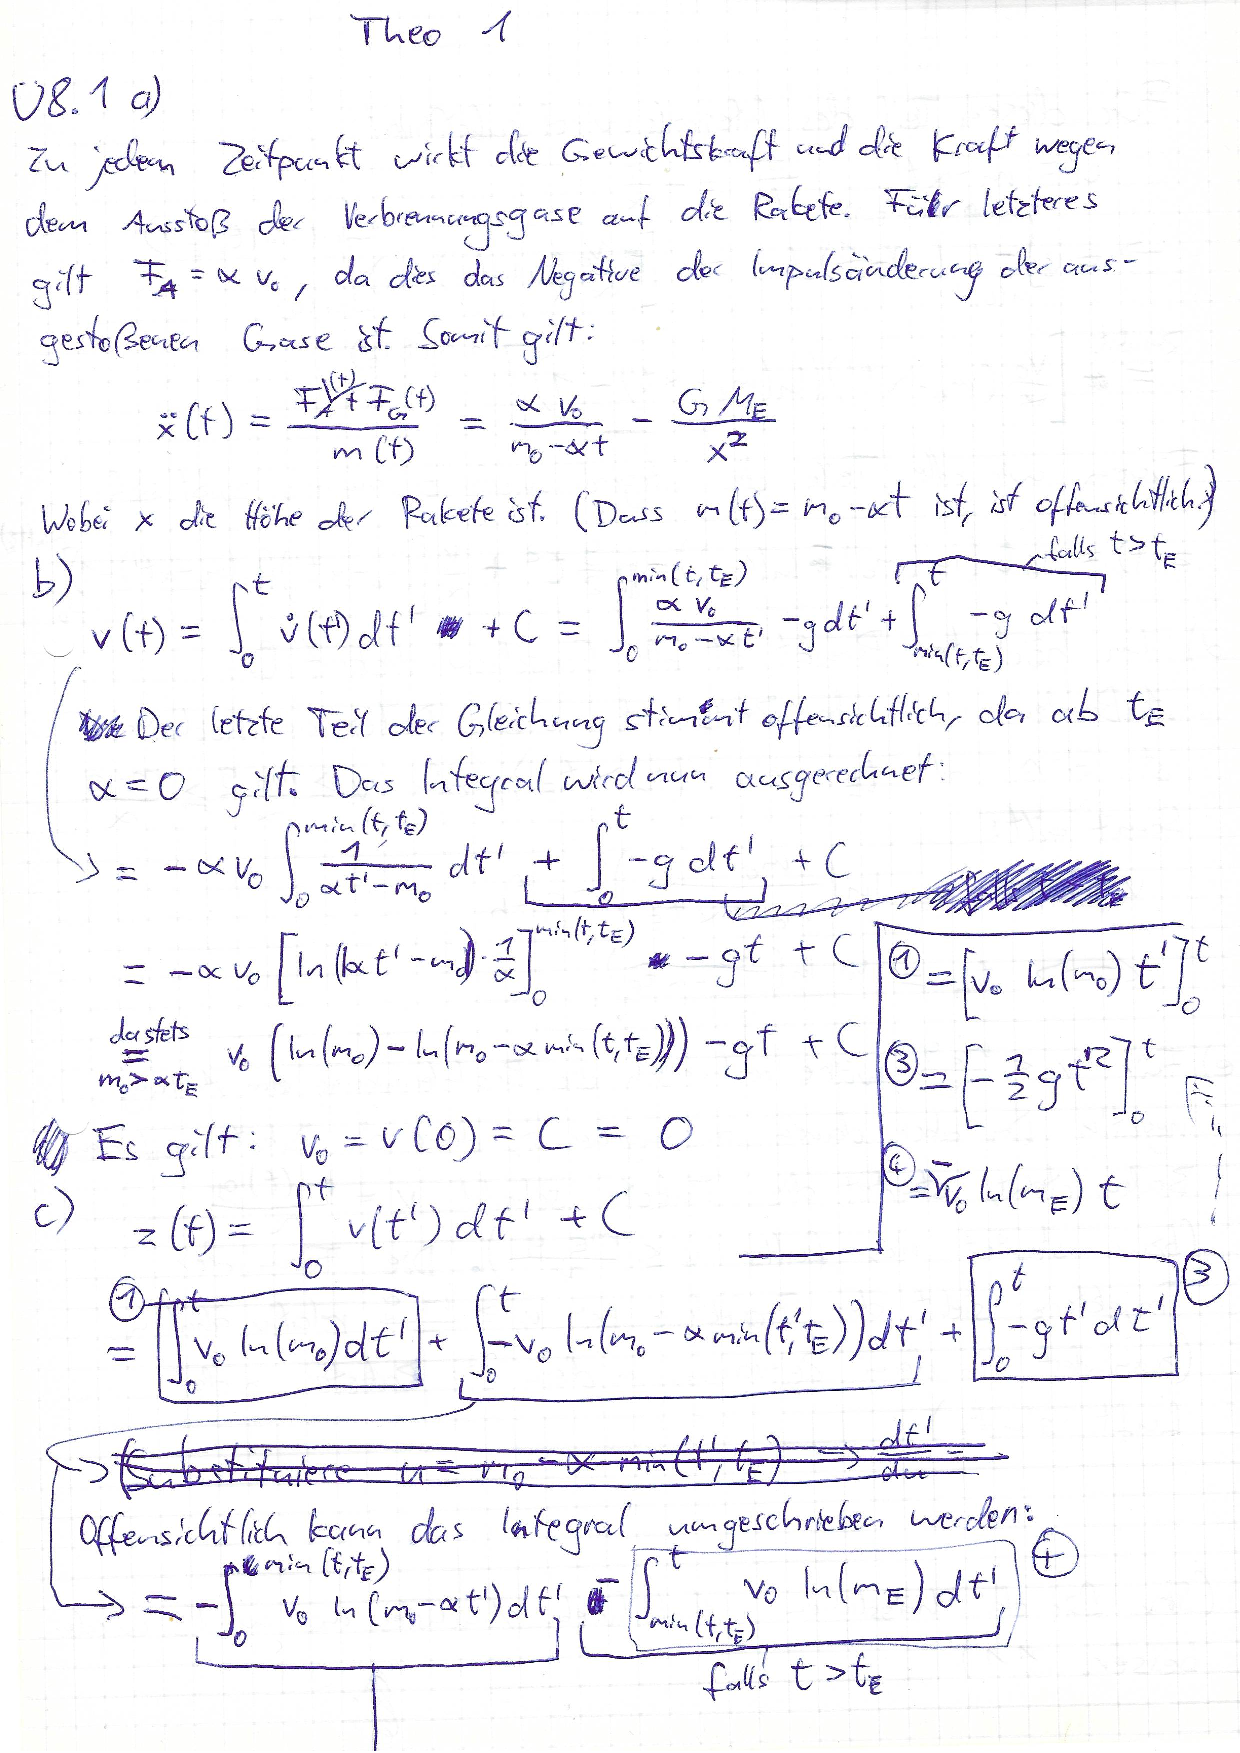
\includepdf[pages=-, pagecommand={\thispagestyle{plain}}]{Theo1U8A1.pdf}


\section*{Aufgabe 8.2}	
\begin{center}
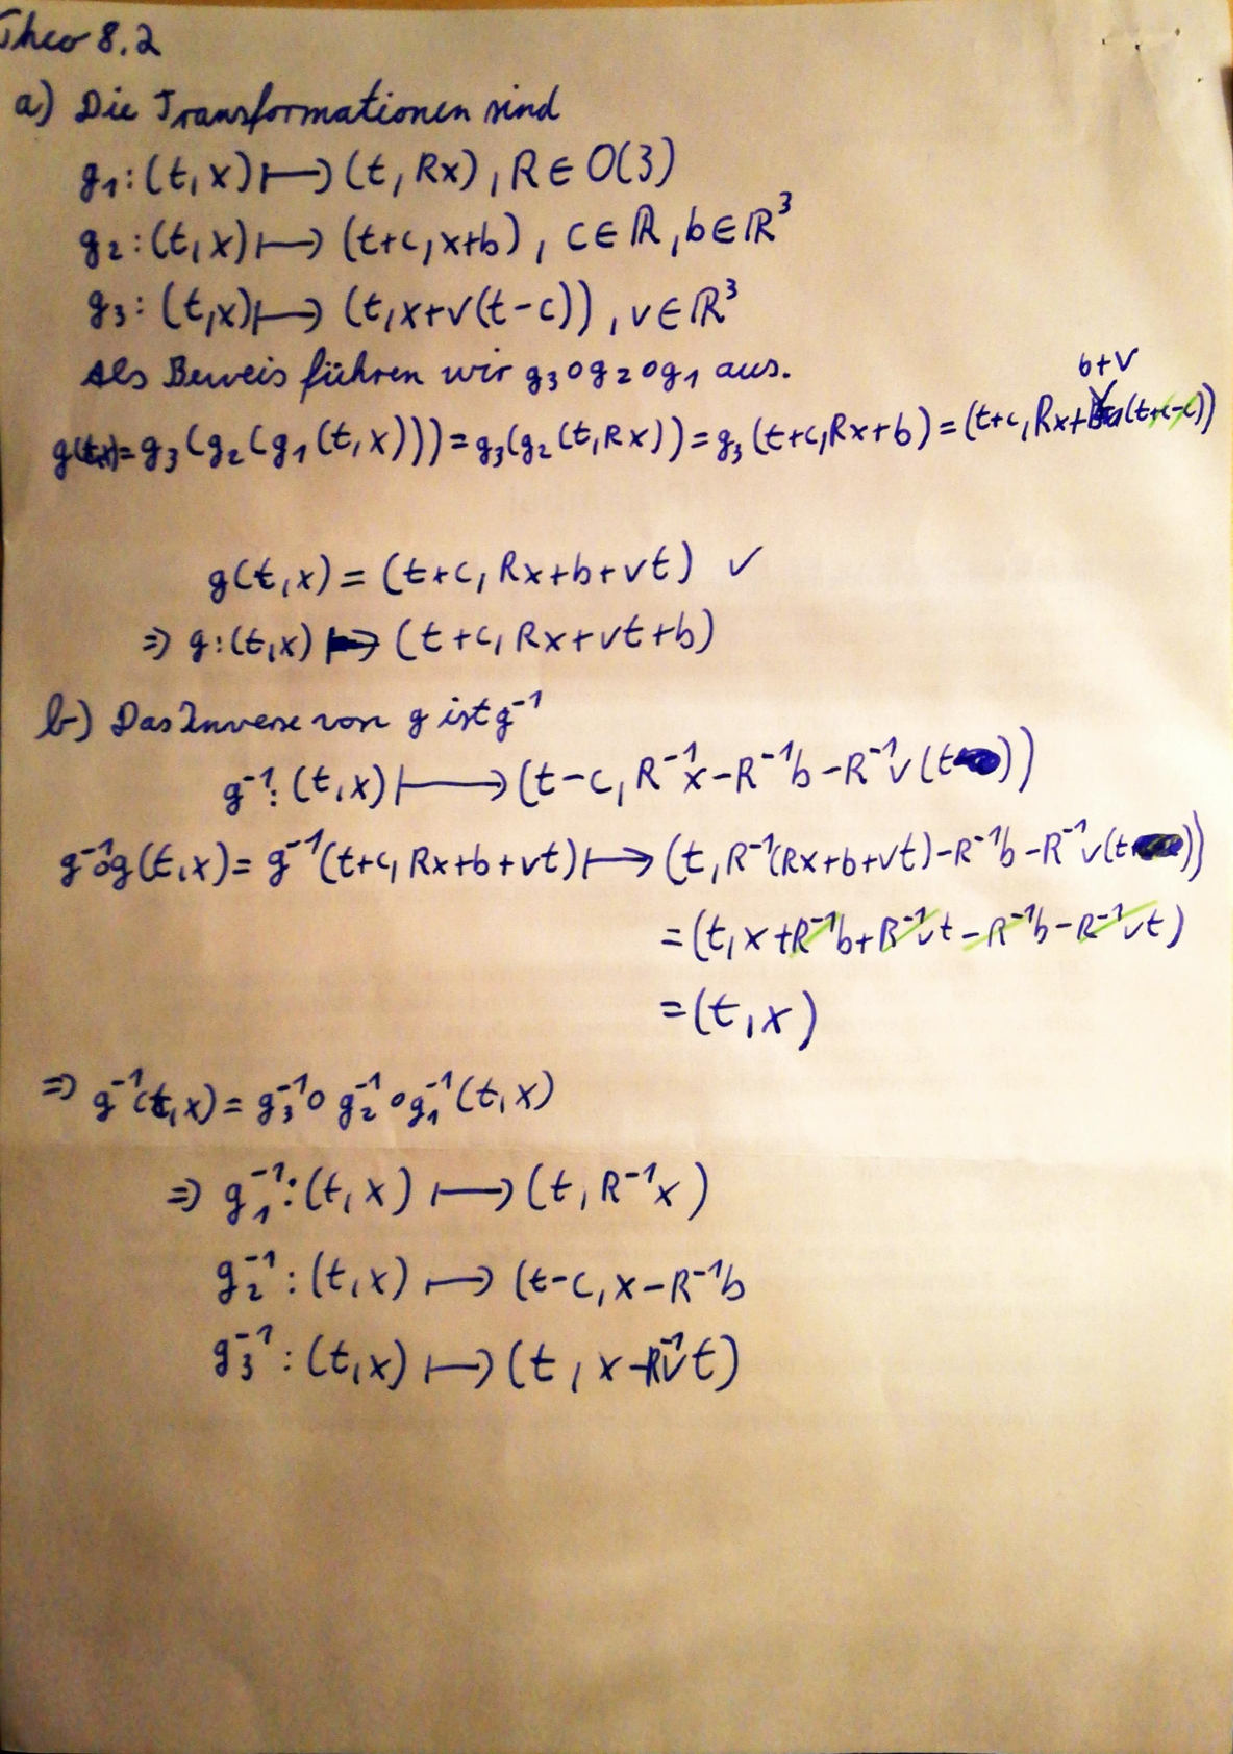
\includegraphics[width=14cm]{PTP8-2)_1.pdf}
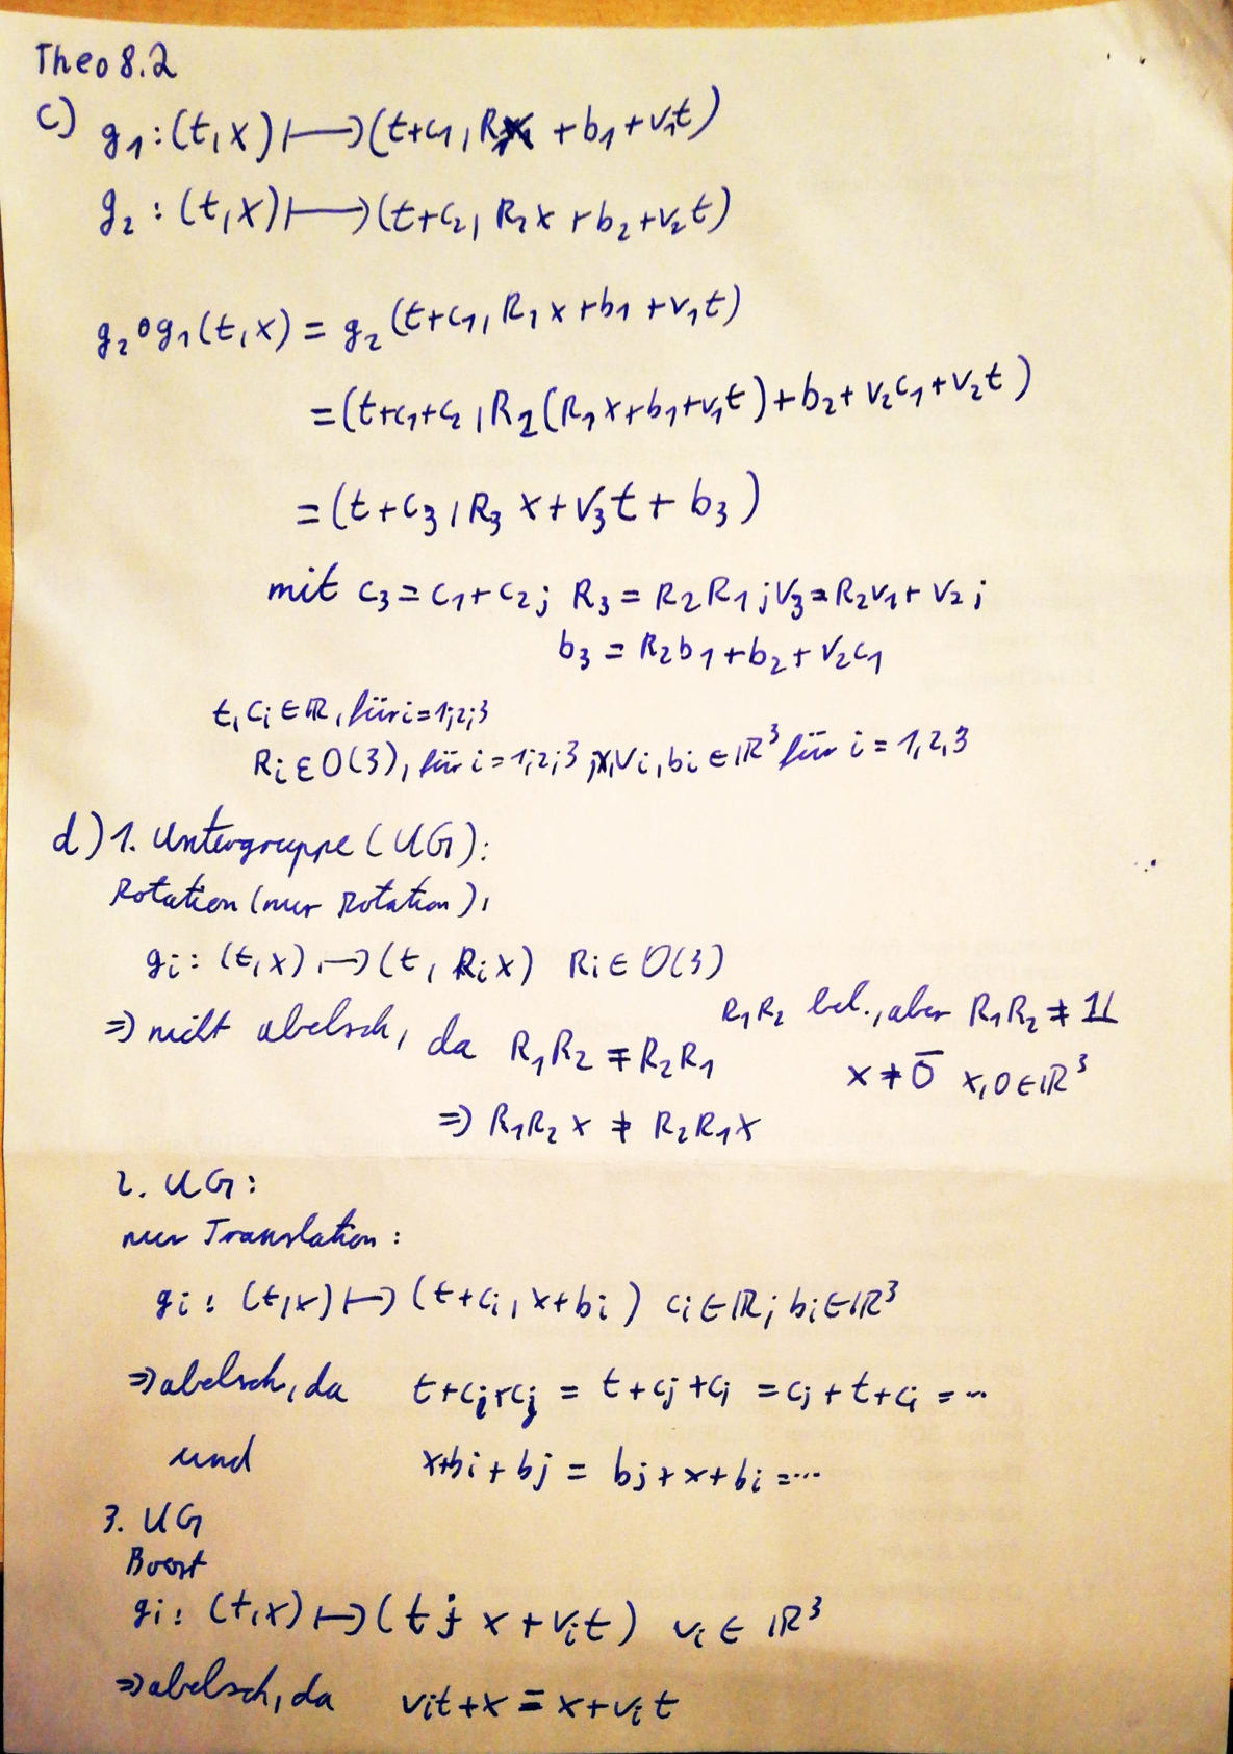
\includegraphics[width=14cm]{PTP8-2)_2.pdf}
\end{center}
\newpage



\end{document}
